\paragraph*{1 - Alphabete, Wörter, Sprachen}

\begin{example2}{Multiple-Choice} $\surd$ = richtig, $\boxtimes$ = falsch
    \begin{itemize}
        \item $\boxtimes$ Konkatenation von Sprachen = Vereinigung der zugrundeliegenden Alphabete
        \item $\boxtimes$ $L = \{\} \equiv K = \{\epsilon\}$
        \item $\boxtimes$ $\epsilon \in AB$ oder $\epsilon100 \in AB$ 
        für $A$ enthält alle Binärwörter die mit 0 enden, $B$ alle die mit 1 enden
    \end{itemize}
\end{example2}

\paragraph*{2 - Reguläre Ausdrücke}

\begin{example2}{Reguläre Ausdrücke und Sprachen}
    \begin{itemize}
        \item $\epsilon$ = Sprache aller Binärzahlen Länge 0
        \item $(1(0 \mid 1)*1) \mid 1$ = Sprache aller positiver ungerader Binärzahlen
        \item $(0 \mid 0001)*$ = Sprache aller Wörter die vor jeder 1 mind. 3 Nullen haben
        \item $(0 \mid 1)*0(0 \mid 1)*0(0 \mid 1)*0(0 \mid 1)*$ = Sprache aller Binärzahlen die mind. 4 Nullen enthalten
    \end{itemize}

    \vspace{2mm}

    regulär/nicht regulär:
    \begin{itemize}
        \item $\{(it)^n \mid n \in \N\} \rightarrow$ regulär
        \item $\{w \in {a,b}* \mid a^m b^n \text { mit } m \neq n\} \rightarrow$ nicht regulär
        \item Windows Dateinamen $\rightarrow$ regulär
        \item Sprache der Wörter mit doppelt so vielen 0 wie 1 $\rightarrow$ nicht regulär
    \end{itemize}
\end{example2}

\paragraph*{3 - Endliche Automaten}


\begin{example2}{Zustandsklassen} {\small EA akzeptiert Binärwörter wo $|0|$ und $|1|$ gerade}

    \begin{minipage}
        {0.3\linewidth}
        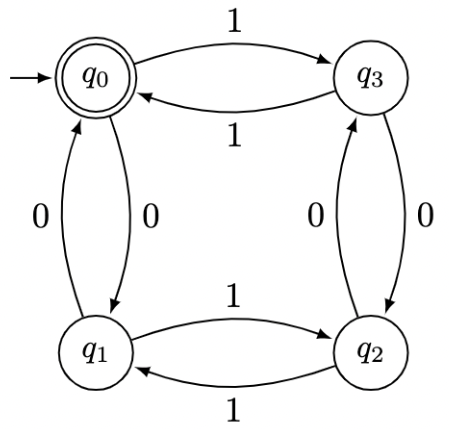
\includegraphics[width=1\linewidth]{images/zustandbsp.png}
    \end{minipage}
    \begin{minipage}{0.7\linewidth}
        
        Klasse $[q_0] = \{w \in \{0,1\}^* \mid |w|_0 = 2i \text{ und } |w|_1 = 2j \text{ für } i,j \in \N\}$

        Klasse $[q_1] = \{w \in \{0,1\}^* \mid |w|_0 = 2i+1 \text{ und } |w|_1 = 2j \text{ für } i,j \in \N\}$

        Klasse $[q_2] = \{w \in \{0,1\}^* \mid |w|_0 = 2i+1 \text{ und } |w|_1 = 2j+1 \text{ für } i,j \in \N\}$

        Klasse $[q_3] = \{w \in \{0,1\}^* \mid |w|_0 = 2i \text{ und } |w|_1 = 2j+1 \text{ für } i,j \in \N\}$
        
    \end{minipage}

    {\small $0 \Rightarrow i$, $1 \Rightarrow j$}
\end{example2}

\begin{example2}{Widerspruchsbeweis}
   dass jeder deterministische endliche Automat für die Sprache:
$
L=\left\{w \in\{a, b\}^* \mid w \text { hat den Suffix ab }\right\}
$
mindestens 3 Zustände braucht.

Für den Widerspruchsbeweis wählen wir die folgenden Wörter: $x_1=[\varepsilon], x_2=a, x_3=ab$

Widerspruch für alle Wortpaare:

$
\begin{aligned}
& x_1 \text { und } x_2: \quad[\mathrm{z} 12]=[\mathrm{b}] \Rightarrow[\mathrm{x} 1][\mathrm{z} 12]=[\mathrm{b}] \notin L, \quad[\mathrm{x} 2][\mathrm{z} 12]=[\mathrm{ab}] \in L \\
& x_1 \text { und } x_3: \quad[\mathrm{z} 13]=[\varepsilon] \Rightarrow[\mathrm{x} 1][\mathrm{z} 13]=[\varepsilon] \notin L, \quad[\mathrm{x} 3][\mathrm{z} 13]=[\mathrm{ab}] \in L \\
& x_2 \text { und } x_3: \quad[\mathrm{z} 23]=[\varepsilon] \Rightarrow[\mathrm{x} 2][\mathrm{z} 23]=[\mathrm{a}] \notin L, \quad[\mathrm{x} 3][\mathrm{z} 23]=[\mathrm{ab}] \in L \\
&
\end{aligned}
$
\end{example2}

\begin{example2}{Sprachen in EA umwandelbar}

    $
L=\{w \in\{0,1\}^* \mid w=0^n 10^n \text { und } n \in \mathbb{N}\}
$
: DEA nicht möglich

$
L=\{w \in\{0,1\}^*|| w|_1 \leq 3\}
$
: DEA möglich

$
L=\{w \in\{0,1\}^* \mid w=0^* 10^*\}
$
: DEA möglich

$
L=\{\boldsymbol{w} \in\{0,1\}^* \mid w=0^n 1^m 0 \text { und } n, m \in \mathbb{N}\}
$
: DEA möglich

$
L=\{w \in\{0,1\}^*|| w|_0=|w|_1\}
$
: DEA nicht möglich
\end{example2}

\paragraph{KFG}

\begin{minipage}{0.8\linewidth}
\begin{example2}{Ableitungsbaum für Grammatik der Chemie}

    Vereinfachtes bsp über das Wort $ThI_2N*$

    $G_{\text {Chem }}=\{\{S, E, D\},\{T h, I, N, 2\}, P, S\} \text { mit } P=\{ \\  \quad S \rightarrow S E \mid E, \\  \quad E \rightarrow E D|T h| I \mid N, \\  \quad D \rightarrow 2 \quad \}$

    \vspace{1mm}

    Rechtsseitige Ableitung: $S \rightarrow S E \rightarrow S N \rightarrow S E N \rightarrow S E D N \rightarrow S E 2 N \rightarrow S I 2 N \rightarrow E I 2 N \rightarrow$ ThI $2 N$

    \vspace{1mm}

    Beweis Eindeutigkeit: Die kontextfreie Grammatik ist eindeutig, da es immer nur einen Ableitungsbaum gibt (nur einen Pfad der Rekursion möglich, $S$ immer nur $\rightarrow S E$ und $E$ immer nur $\rightarrow E D$ ).
\end{example2}
\end{minipage}
\begin{minipage}{0.2\linewidth}
    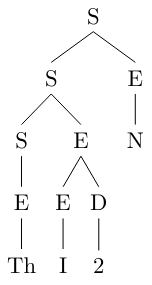
\includegraphics[width=1\linewidth]{images/ableitungsbaum_bsp.png}
\end{minipage}

\begin{example2}{Grammatikaussagen}
    Betrachten Sie die folgenden zwei kontextfreien Grammatiken über dem gegebenen Alphabet $\Sigma=\{0,1\}$
$$
\begin{aligned}
& K_1=\{\{S\}, \Sigma, P_1, S\} \text { mit } P_1=\{S \rightarrow 0 S 1, S \rightarrow 01, S \rightarrow \epsilon\} \\
& K_2=\{\{S, A\}, \Sigma, P_2, S\} \text { mit } P_2=\{S \rightarrow 0 A, A \rightarrow A 1 \mid \epsilon\}
\end{aligned}
$$
Entscheiden Sie, für welche Sprachen die Grammatikaussagen zustimmen:
[K1] erzeugt die Sprache von Wörtern, in denen auf $\boldsymbol{n}$ Nullen $\boldsymbol{n}$ Einsen folgen.
[K2] erzeugt die Sprache von Wörtern, in denen einer Null beliebig viele Einsen folgen.

Entscheiden Sie, mit welchen Grammatiken die folgenden Sprachen gebildet werden können:

$
\begin{aligned}
& S_1=\{w \in\{0,1\}^{\star} \mid w=0^n 1^n \wedge n \in \mathbb{N}\}[\mathrm{K} 1] \\
& S_2=\{w \in\{0,1\}^{\star} \mid w=01^n \wedge n \in \mathbb{N}\}[\mathrm{K} 2] \\
& S_3=\{w \in\{0,1\}^{\star}|| w|_1>|w|_0\}[\text { Keines] } \\
& S_4=\{w \in\{0,1\}^{\star}|| w|_1<|w|_0\}[\text { Keines] } \\
& S_5=\{w \in\{0,1\}^{\star}|| w|_0=0 \wedge|w|_1=0\}[\mathrm{K} 1] \\
& S_6=\{01\}[\mathrm{K} 1 \text { und K2] }
\end{aligned}
$
\end{example2}

\paragraph{Kellerautomaten und Turingmaschinen}

\begin{example2}{Multiple-Choice} $\surd$ = richtig, $\boxtimes$ = falsch
    \begin{itemize}
        \item $\surd$ Kellerautomat kann mit leerem Keller akzeptieren
        \item $\boxtimes$ Eingabealphabet können, müssen aber nicht identisch sein 
        \item $\surd$ Eine korrekt programmierte Turing-Maschine hält in jedem Fall an, wegen der Bedingung der endlich viele Einsen auf einer Seite
        \item $\surd$ Die Turing Machine wird immer zuerst die Seite mit den endlich vielen Einsen bestimmen. Ansonsten wird sie nicht terminieren
        \item $\boxtimes$ Der Algorithmus, 1 nach rechts, 2 nach links, 3 nach rechts, usw., kann nicht verwendet werden, um zu bestimmen, welche Seite unendlich viele Einsen enthält
        \item $\surd$ Die Turing-Maschine kann bestimmen, ob eine Seite unendlich viele Einsen enthält, wenn eine Seite endlich viele Einsen enthält
    \end{itemize}
\end{example2}


\begin{example2}
    {TM} $M=(\{q_1, q_2, q_3, q_4\},\{0,1\},\{0,1, \cup, a, b\}, \delta, q_1, \cup,\{q_2\})$ 
    
    \begin{minipage}{0.35\linewidth}
    $
    \begin{aligned}
    & \delta(q_1, 1)=(q_4, 1, R), \\
    & \delta(q_4, 0)=(q_3, 0, R), \\
    & \delta(q_4, \cup)=(q_2, a, R), \\
    & \delta(q_3, 1)=(q_4, b, R), \\
    & \delta(q_3, 0)=(q_1, 0, R)
    \end{aligned}
    $
\end{minipage}
\begin{minipage}{0.6\linewidth}
    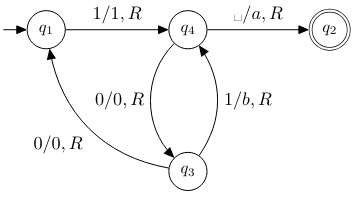
\includegraphics[width=0.9\linewidth]{images/turingmaschine_bsp.png}
\end{minipage}
\end{example2}


\begin{example2}{Busy-Beaver} 
    
    \begin{minipage}{0.4\linewidth}
    terminierende TM, versucht grösstmögliche Ausgabe zu generieren (fixe Anzahl Zustände/Symbolen auf Band)
    \end{minipage}
    \begin{minipage}{0.6\linewidth}
    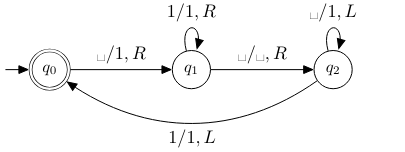
\includegraphics[width=1\linewidth]{images/busybeaver.png}
    \end{minipage}

    \vspace{2mm}

    \begin{minipage}{0.6\linewidth}
        Keller:

        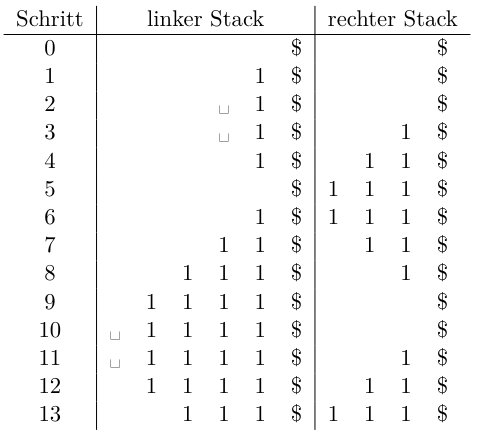
\includegraphics[width=1\linewidth]{images/bbkeller.png}
    \end{minipage}
    \begin{minipage}{0.25\linewidth}
        Band:
        
        \vspace{1mm}

        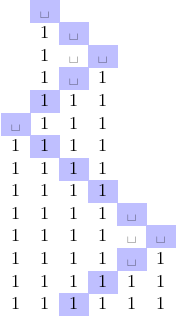
\includegraphics[width=1\linewidth]{images/busybeaverband.png}
    \end{minipage}
\end{example2}

\begin{example2}{Kellerautomat} $L=\{w \in \{0,1\}^{*} \mid |w|_0 < |w|_1\}$

    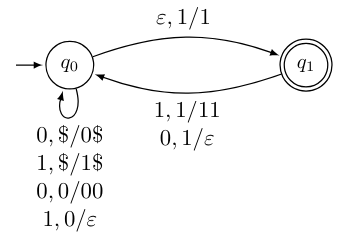
\includegraphics[width=0.4\linewidth]{images/KA_bsp.png}
    
\end{example2}

\begin{example2}{Polynomzeit-Verifizierer}
    Gegeben: $a_1, ... , a_n \in \N$ und $b$

    Ausgabe: JA falls $\exists S \subseteq \{a_1, ... , a_n\}$ mit $\sum_{a_i \in S} a_i = b$, sonst NEIN

    \vspace{2mm}

    Zeuge: konkrete Menge $a_1, ... , a_n \in \N$

    Verifizierer: prüft ob $\sum_{a_i \in S} a_i = b$

    Nur $a_i \in S$ prüfen, da $a_i \notin S$ nicht zur Lösung beiträgt

    Eingabe für Verifizierer: $w = (a_1 1 a_2 1 ... 1 a_n \# b)$
    mit $a_i$ und $b$ unär codiert (z.B. $a_i = 5$ als 00000)

    \vspace{2mm}

    Informell:
    $m$ ist die Länge der Eingabe insgesamt $\rightarrow a_1 1 a_2 1 \ldots 1 a_n \# b$ (Zahlen $a_1, a_2, \ldots, a_n$ und $b$ ). Für die Länge der Eingabe $m$ gilt: max. n Zahlen endlicher Länge + n-mal die „1" $+\mathrm{b}$ mit endlicher Länge (bzw. n Zahlen endlicher Länge) $\Rightarrow$ Länge $(2 m) \in \mathcal{O}(n)$
    
\end{example2}













